% -*- Mode:TeX -*-

%% IMPORTANT: The official thesis specifications are available at:
%%            http://libraries.mit.edu/archives/thesis-specs/
%%
%%            Please verify your thesis' formatting and copyright
%%            assignment before submission.  If you notice any
%%            discrepancies between these templates and the 
%%            MIT Libraries' specs, please let us know
%%            by e-mailing thesis@mit.edu

%% The documentclass options along with the pagestyle can be used to generate
%% a technical report, a draft copy, or a regular thesis.  You may need to
%% re-specify the pagestyle after you \include  cover.tex.  For more
%% information, see the first few lines of mitthesis.cls. 

%\documentclass[12pt,vi,twoside]{mitthesis}
%%
%%  If you want your thesis copyright to you instead of MIT, use the
%%  ``vi'' option, as above.
%%
%\documentclass[12pt,twoside,leftblank]{mitthesis}
%%
%% If you want blank pages before new chapters to be labelled ``This
%% Page Intentionally Left Blank'', use the ``leftblank'' option, as
%% above. 

\documentclass[12pt,twoside]{mitthesis}
\usepackage{lgrind}
%% These have been added at the request of the MIT Libraries, because
%% some PDF conversions mess up the ligatures.  -LB, 1/22/2014
\usepackage{cmap}
\usepackage[T1]{fontenc}
\pagestyle{plain}
\usepackage{graphicx}
\usepackage{amssymb}
\usepackage{amsmath}
\usepackage{calc}
\usepackage{supertabular}
\usepackage{subfigmat}
\usepackage{array}
\usepackage{textcomp}
\usepackage{hyperref}
\usepackage[acronym]{glossaries}
\makeglossaries

%% Create hyperlinks
\usepackage{hyperref}
\hypersetup{
    colorlinks,
    citecolor=black,
    filecolor=black,
    linkcolor=black,
    urlcolor=black
}
%%
\newacronym{CE}{CE}{Convex Engineering}
\newacronym{CEG}{CEG}{Convex Engineering Group}
\newacronym{GP}{GP}{Geometric Programming}
\newacronym{gp}{GP}{Geometric Program}
\newacronym{SP}{SP}{Signomial Programming}
\newacronym{sp}{SP}{Signomial Program}
\newacronym{mdo}{MDO}{Multidisciplinary Design Optimization}
\newacronym{NLP}{NLP}{Nonlinear Programming}

\begin{document}

%% -*-latex-*-
% 
% For questions, comments, concerns or complaints:
% thesis@mit.edu
% 
%
% $Log: cover.tex,v $
% Revision 1.8  2008/05/13 15:02:15  jdreed
% Degree month is June, not May.  Added note about prevdegrees.
% Arthur Smith's title updated
%
% Revision 1.7  2001/02/08 18:53:16  boojum
% changed some \newpages to \cleardoublepages
%
% Revision 1.6  1999/10/21 14:49:31  boojum
% changed comment referring to documentstyle
%
% Revision 1.5  1999/10/21 14:39:04  boojum
% *** empty log message ***
%
% Revision 1.4  1997/04/18  17:54:10  othomas
% added page numbers on abstract and cover, and made 1 abstract
% page the default rather than 2.  (anne hunter tells me this
% is the new institute standard.)
%
% Revision 1.4  1997/04/18  17:54:10  othomas
% added page numbers on abstract and cover, and made 1 abstract
% page the default rather than 2.  (anne hunter tells me this
% is the new institute standard.)
%
% Revision 1.3  93/05/17  17:06:29  starflt
% Added acknowledgements section (suggested by tompalka)
% 
% Revision 1.2  92/04/22  13:13:13  epeisach
% Fixes for 1991 course 6 requirements
% Phrase "and to grant others the right to do so" has been added to 
% permission clause
% Second copy of abstract is not counted as separate pages so numbering works
% out
% 
% Revision 1.1  92/04/22  13:08:20  epeisach

% NOTE:
% These templates make an effort to conform to the MIT Thesis specifications,
% however the specifications can change.  We recommend that you verify the
% layout of your title page with your thesis advisor and/or the MIT 
% Libraries before printing your final copy.
\title{Conceptual Engineering Design and Optimization Methodologies using Geometric Programming}


\author{Berk Ozturk}
% If you wish to list your previous degrees on the cover page, use the 
% previous degrees command:
%       \prevdegrees{A.A., Harvard University (1985)}
% You can use the \\ command to list multiple previous degrees
%       \prevdegrees{B.S., University of California (1978) \\
%                    S.M., Massachusetts Institute of Technology (1981)}
\department{Department of Aeronautics and Astronautics}

% If the thesis is for two degrees simultaneously, list them both
% separated by \and like this:
% \degree{Doctor of Philosophy \and Master of Science}
\degree{Master of Science in Aeronautics and Astronautics}

% As of the 2007-08 academic year, valid degree months are September, 
% February, or June.  The default is June.
\degreemonth{Febrary}
\degreeyear{2018}
\thesisdate{February 1st, 2018}

%% By default, the thesis will be copyrighted to MIT.  If you need to copyright
%% the thesis to yourself, just specify the `vi' documentclass option.  If for
%% some reason you want to exactly specify the copyright notice text, you can
%% use the \copyrightnoticetext command.  
%\copyrightnoticetext{\copyright IBM, 1990.  Do not open till Xmas.}

% If there is more than one supervisor, use the \supervisor command
% once for each.
\supervisor{Mark Drela}{Professor, Aeronautics and Astronautics}

% This is the department committee chairman, not the thesis committee
% chairman.  You should replace this with your Department's Committee
% Chairman.
\chairman{Hamsa Balakrishnan}{Associate Professor, Aeronautics and Astronautics\\
Chair, Graduate Program Committee}

% Make the titlepage based on the above information.  If you need
% something special and can't use the standard form, you can specify
% the exact text of the titlepage yourself.  Put it in a titlepage
% environment and leave blank lines where you want vertical space.
% The spaces will be adjusted to fill the entire page.  The dotted
% lines for the signatures are made with the \signature command.
\maketitle

% The abstractpage environment sets up everything on the page except
% the text itself.  The title and other header material are put at the
% top of the page, and the supervisors are listed at the bottom.  A
% new page is begun both before and after.  Of course, an abstract may
% be more than one page itself.  If you need more control over the
% format of the page, you can use the abstract environment, which puts
% the word "Abstract" at the beginning and single spaces its text.

%% You can either \input (*not* \include) your abstract file, or you can put
%% the text of the abstract directly between the \begin{abstractpage} and
%% \end{abstractpage} commands.

% First copy: start a new page, and save the page number.
\cleardoublepage
% Uncomment the next line if you do NOT want a page number on your
% abstract and acknowledgments pages.
% \pagestyle{empty}
\setcounter{savepage}{\thepage}
\begin{abstractpage}
% $Log: abstract.tex,v $
% Revision 1.1  93/05/14  14:56:25  starflt
% Initial revision
% 
% Revision 1.1  90/05/04  10:41:01  lwvanels
% Initial revision
% 
%
%% The text of your abstract and nothing else (other than comments) goes here.
%% It will be single-spaced and the rest of the text that is supposed to go on
%% the abstract page will be generated by the abstractpage environment.  This
%% file should be \input (not \include 'd) from cover.tex.


Geometric programs (GPs) and other forms of convex optimization have recently experienced
a resurgence due to polynomial-time solution algorithms and improvements in computing.
Observing the need for fast and stable methods for multidisciplinary
design optimization (MDO),
previous work has shown that geometric programming can be a powerful framework
for MDO by leveraging the mathematical guarantees
and speed of convex optimization. However, there exists a variety of barriers for
implementing optimization in design. In this work, we formalize why the formulation
of general non-linear design problems as GPs facilitates design. By systematically
formulating an aircraft design problem from core physical principles, we present methods
to convert non-linear constraints and data-based relations into GP-compatible forms,
and demonstrate the benefits of the difference-of-convex extension of
GPs called signomial programs (SPs).
The extensibility of GP models is demonstrated through an expansion
in the fidelity of the model.
The features specific to GPkit, an object-oriented GP model formulation framework, in
facilitating the modern engineering design process are demonstrated.
Using both performance and mission modeling paradigms, we demonstrate the ability to
model and design complex systems in GP, and extract maximal engineering intuition
using sensitivities and tradespace exploration methods.
Though the methods are applied to an aircraft design problem, they are general to
models with continuous, explicit constraints, and help lower the barriers to implementing
optimization in design.


\end{abstractpage}

% Additional copy: start a new page, and reset the page number.  This way,
% the second copy of the abstract is not counted as separate pages.
% Uncomment the next 6 lines if you need two copies of the abstract
% page.
% \setcounter{page}{\thesavepage}
% \begin{abstractpage}
% % $Log: abstract.tex,v $
% Revision 1.1  93/05/14  14:56:25  starflt
% Initial revision
% 
% Revision 1.1  90/05/04  10:41:01  lwvanels
% Initial revision
% 
%
%% The text of your abstract and nothing else (other than comments) goes here.
%% It will be single-spaced and the rest of the text that is supposed to go on
%% the abstract page will be generated by the abstractpage environment.  This
%% file should be \input (not \include 'd) from cover.tex.


Geometric programs (GPs) and other forms of convex optimization have recently experienced
a resurgence due to polynomial-time solution algorithms and improvements in computing.
Observing the need for fast and stable methods for multidisciplinary
design optimization (MDO),
previous work has shown that geometric programming can be a powerful framework
for MDO by leveraging the mathematical guarantees
and speed of convex optimization. However, there exists a variety of barriers for
implementing optimization in design. In this work, we formalize why the formulation
of general non-linear design problems as GPs facilitates design. By systematically
formulating an aircraft design problem from core physical principles, we present methods
to convert non-linear constraints and data-based relations into GP-compatible forms,
and demonstrate the benefits of the difference-of-convex extension of
GPs called signomial programs (SPs).
The extensibility of GP models is demonstrated through an expansion
in the fidelity of the model.
The features specific to GPkit, an object-oriented GP model formulation framework, in
facilitating the modern engineering design process are demonstrated.
Using both performance and mission modeling paradigms, we demonstrate the ability to
model and design complex systems in GP, and extract maximal engineering intuition
using sensitivities and tradespace exploration methods.
Though the methods are applied to an aircraft design problem, they are general to
models with continuous, explicit constraints, and help lower the barriers to implementing
optimization in design.


% \end{abstractpage}

\cleardoublepage

\section*{Acknowledgments}

Firstly, I would like to thank Professor Warren Hoburg for giving me
the opportunity to work on research that I believe has great potential.
He introduced me to geometric programming and welcomed me to the Hoburg Research Group
(now the Convex Engineering Group). Under his mentorship, I learned that the most interesting designs
are the ones we don't expect, and that challenging current engineering design methods and norms
is the most worthwhile objective of optimization.
So thank you for the opportunity to do just that.

I am grateful for the many friends I have in the Aerospace Computational Design
Lab (ACDL) who have made lightened my work hours with their camaraderie. Of this group,
the Convex folks reserve a special place. I am lucky to collaborate with
such a talented and dedicated group of researchers, and I hope that we will continue
to redefine conceptual engineering design.

This thesis would not have been possible without the amazing work Ned Burnell does
as the lead developer of GPkit. It was prompted by the many debates we have had about
design philosophy,
and I'm glad I've gotten the opportunity to extensively document many of the ideas
that were discussed.
He never ceases to amaze me with his creativity and energy, and I look
forward to future work together.

I thank my co-advisors Professor Mark Drela and Bob Haimes, who have taken on the burden of advising
me in Woody's absence. Thank you for your guidance and wisdom, and pushing me to
finish this thesis.

I am indebted to cycling for keeping me fit and sane, and giving me opportunities to
escape. MIT Cycling has been an immutable source of joy in my life, and I feel proud
every time I put on the grey jersey. MIT Cyclists are near and dear to my heart, and
I look forward to every adventure we have together, on or off the bike.

I would like to thank my flatmate and long-time friend Johannes Norheim
for being a battle-scarred companion through 5 years of MIT. We have been challenged, and
our paths have converged and diverged many times, but our friendship has not wavered.
I anticipate we will continue to survive and thrive at MIT!
My partner Elise Newman has been a ray of sunshine in every weather,
and I am looking forward to our future together.

My parents definitely deserve a mention because I wouldn't exist without them.
The longer I live, the more I understand that I am where I am because of the
sacrifices they have made.
Deniz, you have been my rock. It has been my privilege to be your brother and watch
you grow up, and will be my privilege to help you
through your struggles and celebrate your future successes.
I am confident you will be more than I have been.

%%%%%%%%%%%%%%%%%%%%%%%%%%%%%%%%%%%%%%%%%%%%%%%%%%%%%%%%%%%%%%%%%%%%%%
% -*-latex-*-

% Some departments (e.g. 5) require an additional signature page.  See
% signature.tex for more information and uncomment the following line if
% applicable.
% % -*- Mode:TeX -*-
%
% Some departments (e.g. Chemistry) require an additional cover page
% with signatures of the thesis committee.  Please check with your
% thesis advisor or other appropriate person to determine if such a 
% page is required for your thesis.  
%
% If you choose not to use the "titlepage" environment, a \newpage
% commands, and several \vspace{\fill} commands may be necessary to
% achieve the required spacing.  The \signature command is defined in
% the "mitthesis" class
%
% The following sample appears courtesy of Ben Kaduk <kaduk@mit.edu> and
% was used in his June 2012 doctoral thesis in Chemistry. 

\begin{titlepage}
\begin{large}
This doctoral thesis has been examined by a Committee of the Department
of Chemistry as follows:

\signature{Professor Jianshu Cao}{Chairman, Thesis Committee \\
   Professor of Chemistry}

\signature{Professor Troy Van Voorhis}{Thesis Supervisor \\
   Associate Professor of Chemistry}

\signature{Professor Robert W. Field}{Member, Thesis Committee \\
   Haslam and Dewey Professor of Chemistry}
\end{large}
\end{titlepage}



  % -*- Mode:TeX -*-
%% This file simply contains the commands that actually generate the table of
%% contents and lists of figures and tables.  You can omit any or all of
%% these files by simply taking out the appropriate command.  For more
%% information on these files, see appendix C.3.3 of the LaTeX manual. 
\tableofcontents
\newpage
\listoffigures
\newpage
\listoftables


\chapter{Introduction}

Modern engineering design, and particularly aerospace design, has come to rely
heavily on optimization. Time and time again, the importance of fast and
reliable MDO tools has been stressed in the literature. However most MDO tools
have the downfalls of being slow due to the multimodal nature of many
engineering design problems.
	
In the \gls{CEG}, we seek to improve the engineering design process by
leveraging the mathematical guarantees of convex optimization, and developing
open-source, object-oriented software to help build GP-compatible models and
interface with solvers. In much of our previous work
(\cite{gp_ac_design},\cite{SP_ac_design}, \cite{turbofan}), we have demonstrated that
\gls{GP} is useful for optimization, but have yet to formalize why it
facilitates design.
 
The mathematical restrictions on the form of constraints remains the biggest
barrier in the implementation of convex programs in design. Firstly, this thesis
will aim to show that the form of the GP actually facilitates the design process
and engineering understanding, rather than impeding it. Hence it will aim to
pass on some of the expertise we have developed in the \gls{CEG} building
\gls{GP}-compatible models.

Secondly, it will aim to showcase the features of GPkit in further facilitating
an engineering design process that is streamlined and collaborative, and is
compatible with modern engineering design methodologies (flexibility and
modularity). GPkit allows feedback between design engineers and models (speed
and sensitivities) which allows targeted efforts by engineers to improve models.

(NED Comment: What about conceptual design? Collaboration?)

\section{Defining Design versus Optimization} \label{sec:DesVsOpt}

\subsection{What is design?}

\begin{itemize}
\item To conceive the look (the form) and function of something. 
\item Ned's comment: Parametrization and physics. Hard to agree on a representation that we all agree on. 
\item It is a PROCESS
\begin{itemize}
	\item The 'look' is the configuration
	\item The function is oftentimes what we can quantify
\end{itemize}
\item Essentially a class of feasibility problems, given a set of requirements. 
\end{itemize}

\subsection{What is optimization?}

\begin{itemize}
\item Has a rigorous mathematical definition: The selection of an element in a set 
of feasible solutions with the lowest desired objective function value. 
\item It is also a process!
\item It is sensitive to the choice of objective function, and the elements 
contained within the set (configuration)
\item To many engineers, design and optimization are one and the same. 
\end{itemize}

\subsection{What are the fundamental differences?}

\begin{itemize}
\item Design is human-driven. Optimization is computational. 
\item Design is based on feasibility. Optimization is based on the mathematical guarantees of optimality. 
\item Design can be done in non-restrictive mathematical forms. Optimization is done in specific mathematical forms that take advantage of structure. 
\end{itemize}

\section{Unifying design and optimization using gls{GP}}


\gls{GP} has developed "in response to a need to solve problems in the actual 
world".~\cite{duffingp} Quote from Duffin, 1967, main inventor of GP.

(Each section in this part of the intro has a corresponding section in the body.
(Each will feature an example problem that I will run through as a
(demonstration.)

There are three primary reasons why...

\begin{enumerate}     \item \textit{Inequalities help engineering
understanding.}

The mathematical constraints of \gls{GP} force designers to have a proper grasp
of the fundamental tradeoffs and pressures in a design.

Inequalities make feasible sets explicit. ADD A DIAGRAM OF FEASIBLE SETS using
SimPleAC HERE.

Traditionally, physical relations are expressed as equalities. But there is an
almost-seamless transition from fundamental physics to GP-compatible
constraints. ENGINEERS LIKE +VE QUANTITIES. eg. downforce vs. negative lift.

And even if the tradeoffs are not clear, we can use signomial equalities to
enforce constraints.

    \item \textit{Models are extensible.}
    
Models can be made arbitrarily complex. The 'bag of constraints' form of the GP
means that there is no need to reformulate the optimization scheme as more
constraints are added. This makes incremental modeling improvements possible and
even preferable.

The traditional engineering design process is split into conceptual, preliminary
and critical design segments. GP modeling facilitates this process by allowing
ever-increasing levels of complexity.

Gradient based optimization methods for multimodal systems often involves
converge loops, which have to be reengineered when new constraints are
introduced. VS. adding constraints to a bag...

We can effectively use sensitivity information to determine which parts of the
model yield the greatest returns to improved modeling, so engineers can target
their efforts.

    \item \textit{Models are flexible and modular, and compatible with modern
    engineering design (similar to extensible?)}

(This is a feature of GPkit, and not GPs in general.) \gls{GP}s make it easy to
implement component-based modeling, and build models that are shared between
different design problems. Each component has associated sizing and performance
variables.

This is helped by the fact that underconstrained \gls{GP}s can solve reliably,
and the tightness of constraints can be monitored.

\end{enumerate}




\include{chap2}
\appendix
\section{Geometric Programming}\label{gp_intro}

Introduced in 1967 by Duffin et al.~\cite{duffingp}, a geometric program \gls{GP} is
a type of constrained optimization problem that becomes convex after a
logarithmic change of variables. Modern interior point methods allow a typical
sparse \gls{GP} with tens of thousands of decision variables and tens of thousands of
constraints to be solved in minutes on a desktop computer~\cite{convex}. These
solvers do not require an initial guess, and guarantee convergence to a
\textit{global} optimum, assuming a feasible solution exists. If a feasible
solution does not exist, the solver will return a certificate of infeasibility.
These impressive properties are possible because a GP's objective and
constraints consist of only monomial and posynomial functions, which can be
transformed into convex functions in log space.

A monomial is a function of the form
\begin{equation}\label{e:monomial}
m(\mathbf{u}) = c\prod_{j=1}^{n} u_{j}^{a_{j}}
\end{equation}
where $a_{j} \in \mathbb{R}, c \in \mathbb{R}_{++}$ and $u_{j} \in
\mathbb{R_{++}}$. An example of a monomial is the common expression for lift,
$\frac{1}{2} \rho V^2C_{L}S$. In this case, $\mathbf{u} = (\rho, V, C_{L}, S)$,
$c= 1/2$, and $a = (1, 2, 1, 1)$.

A posynomial is a function of the form
\begin{equation}\label{e:posynomial}
p(\mathbf{u}) = \sum_{k=1}^{K}c_{k}\prod_{j=1}^{n} u_{j}^{a_{jk}}
\end{equation}
where $a_{jk} \in \mathbb{R}, c_{k} \in \mathbb{R}_{++}$ and $u_{j} \in
\mathbb{R_{++}}$. A posynomial is a sum of monomials. Therefore, all monomials
are also one-term posynomials.

A GP minimizes a posynomial objective function subject to monomial equality and
posynomial inequality constraints. A GP written in standard form is

\begin{equation}
\label{e:standardform}
\begin{aligned}
\text{minimize }p_{0}(\mathbf{u})& \\
\text{subject to }p_{i}(\mathbf{u})& \leq 1, i = 1, ...., n_{p}, \\
m_{i}(\mathbf{u})& = 1, i = 1, ..., n_{m}
\end{aligned}
\end{equation}

where $p_{i}$ are posynomial functions, $m_{i}$ are monomial functions, and
$\mathbf{u} \in \mathbb{R}^n_{++}$ are the decision variables. Once a problem
has been formulated in the standard form (Equation \ref{e:standardform}), it can
be solved efficiently.

\section{Signomial Programming}\label{sp_intro}
It is not always possible to formulate a design problem as a GP. This motivates
the introduction of signomials. Signomials have the same form as posynomials
\begin{equation}\label{e:signomial}
s(\mathbf{u}) = \sum_{k=1}^{K}c_{k}\prod_{j=1}^{n} u_{j}^{a_{jk}}
\end{equation}

but the coefficients, $c_{k} \in \mathbb{R}$, can now be any (including
non-positive) real numbers.

A signomial program (SP) is a generalization of GP where the inequality
constraints can be composed of signomial constraints of the form $s(u) \leq 0$..
The log transform of an SP is not a convex optimization problem, but is a
difference of convex optimization problem that can be written in log-space as

\begin{equation}
\begin{aligned}
\text{minimize }f_{0}(\mathbf{x})& \\
\text{subject to }f_{i}(\mathbf{x}) -  g_{i}(\mathbf{x})& \leq 0, i = 1, ...., m
\\
\end{aligned}
\end{equation}

where $f_{i}$ and $g_{i}$ are convex.

There are multiple algorithms that reliably solve signomial programs to
\textit{local} optima \cite{gpintro, spsolutions}. A common solution heuristic,
referred to as difference of convex programming or the convex-concave procedure,
involves solving a sequence of GPs, where each GP is a local approximation to
the SP, until convergence occurs. It is worth noting that the introduction of
even a single signomial constraint to any GP turns the GP into a SP, thus losing
the guarantee of solution convergence to a global optimum. Despite the
possibility of convergence to a local, not global, optimum, SPs are a powerful
tool. The convex approximation, $\hat{f}(x)$, to the non-convex signomial in
log-space, $f(x) - g(x)$, is constructed such that it always satisfies

\begin{equation}
\hat{f}(x) \geq f(x) - g(x) \quad \forall \quad x
\end{equation}

In other words, for each constraint, the feasible set of the convex
approximation $\hat{f}(x) \leq 0$ is a subset of the original SP's feasible set,
$f(x) - g(x) \leq 0$. This means SP inequalities do not require a trust region,
removing the need for trust region parameter tuning and making solving SPs
substantially more reliable than solving general nonlinear programs. Figure
\ref{fig:GPapproxs}, where a series of convex (GP compatible) constraints
approximates a non-convex parabolic drag polar in log space, illustrates this
property.

\begin{figure*}[t!]
    \centering
    \begin{subfigure}[t]{0.5\linewidth}
        \centering
        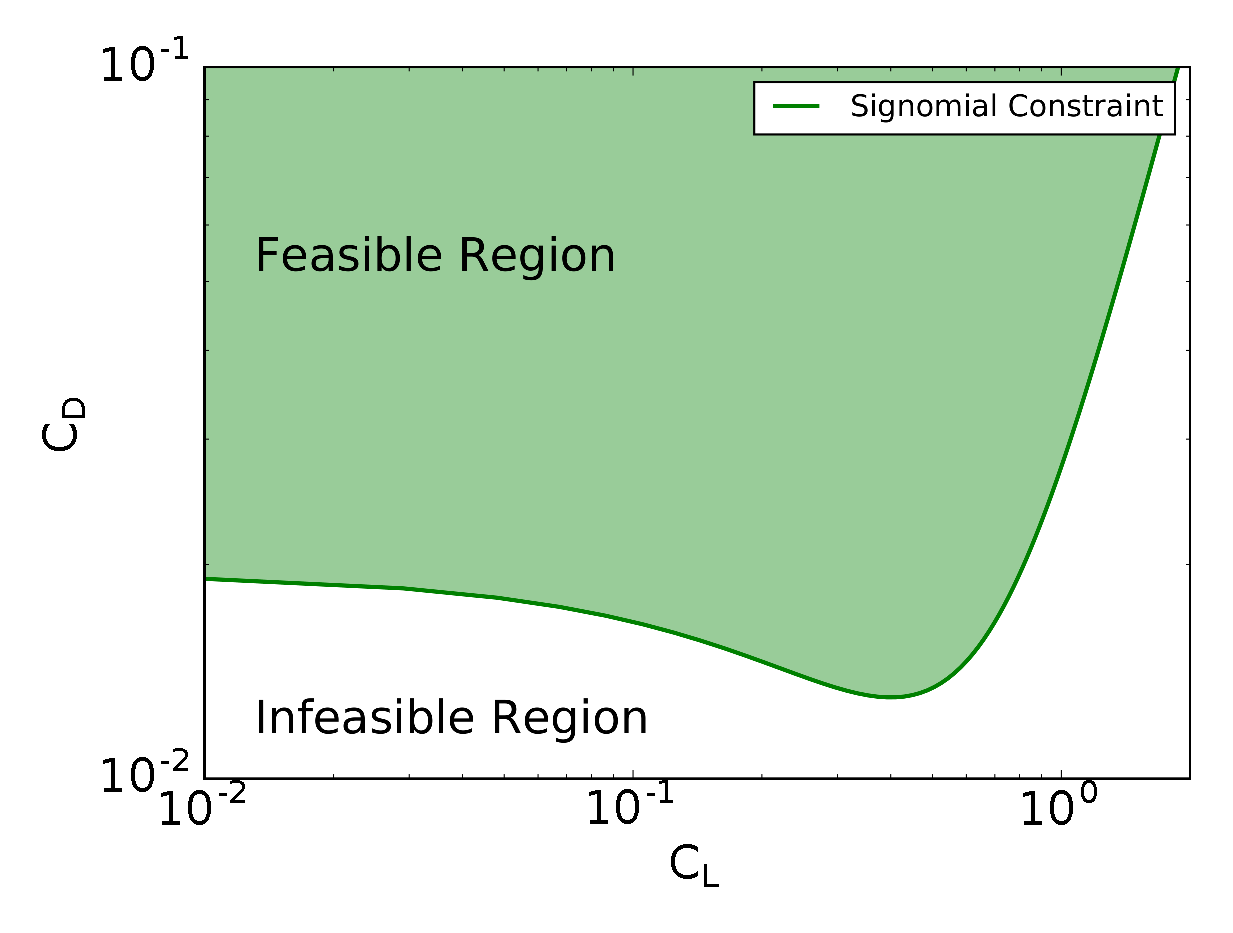
\includegraphics[width=0.9\linewidth]{posyapprox0.eps}
        \caption{Non-convex signomial inequality drag constraint}
    \end{subfigure}%
    ~
    \begin{subfigure}[t]{0.5\linewidth}
        \centering
        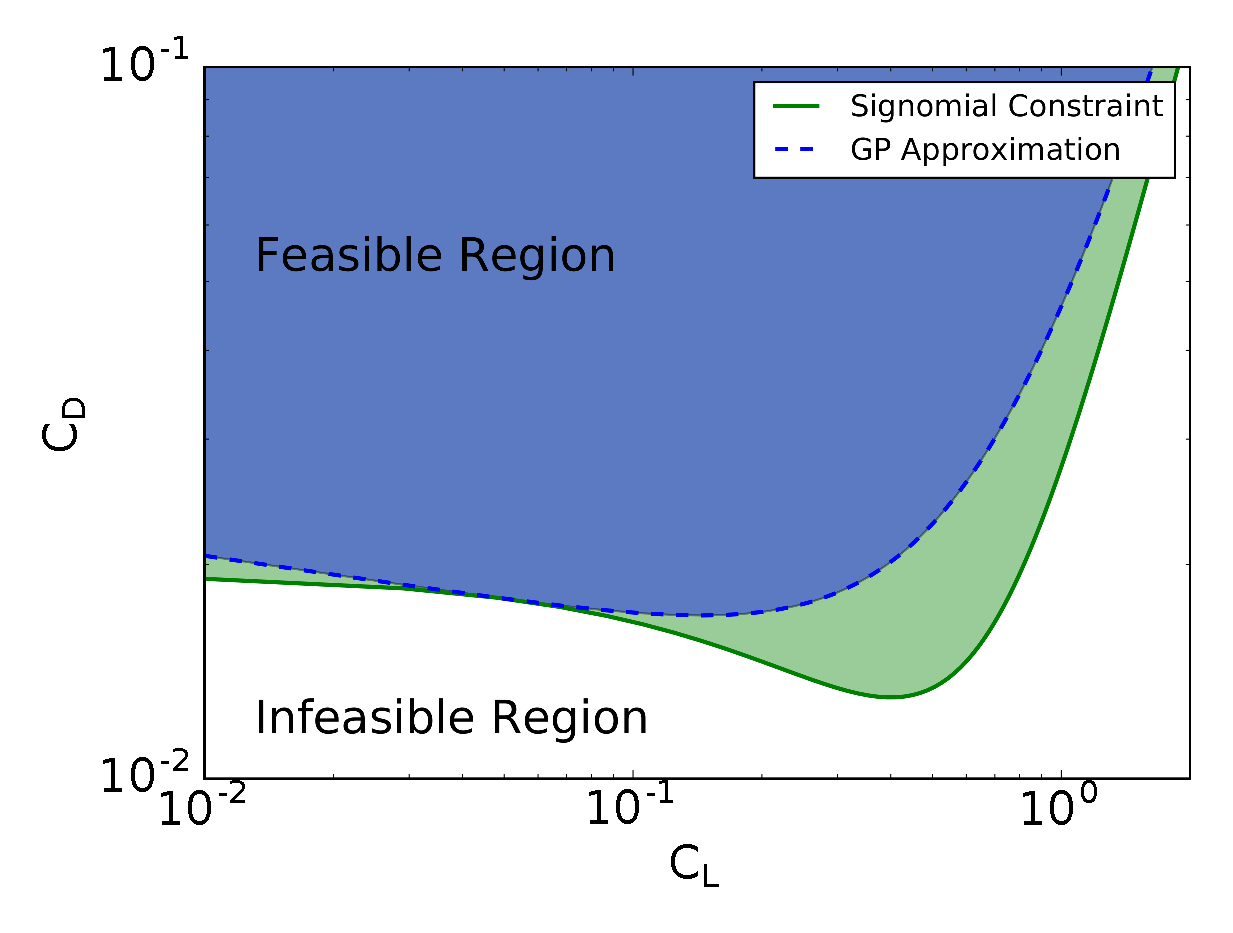
\includegraphics[width=0.9\linewidth]{posyapprox1.eps}
        \caption{Convex approximation about $C_{L} = 0.05$.}
    \end{subfigure}
    \begin{subfigure}[b]{0.5\linewidth}
        \centering
        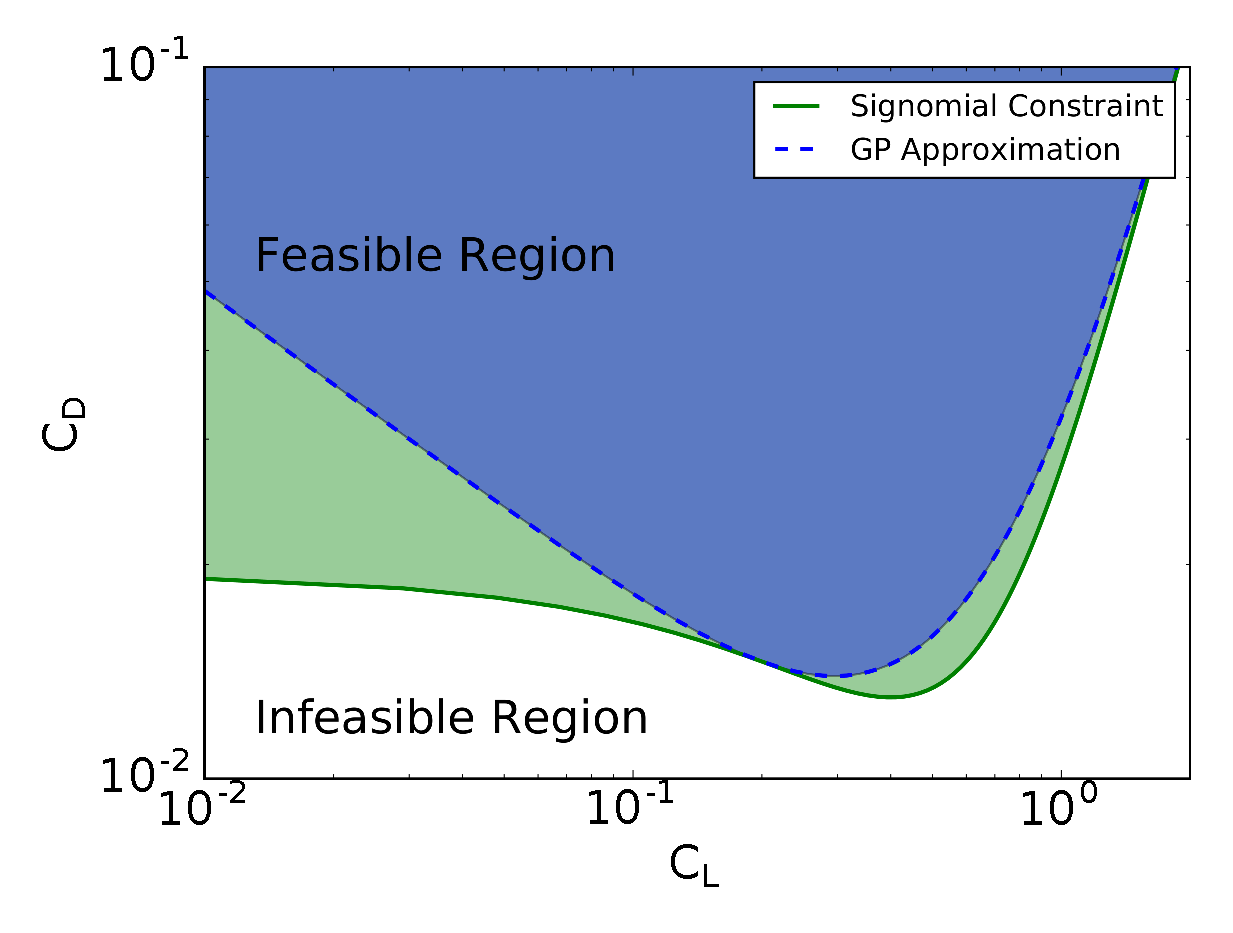
\includegraphics[width=.4\textwidth,natwidth=576,natheight=432]{posyapprox3.eps}
        \caption{Convex approximation about $C_{L} = 0.20.$}
    \end{subfigure}
    \caption{A signomial inequality constraint and GP approximations about two
different points.}
    \label{f:GPapproxs}
\end{figure*}

%\begin{figure}[htbp]
%\centering
%\subfloat[Non-convex signomial inequality drag constraint.]{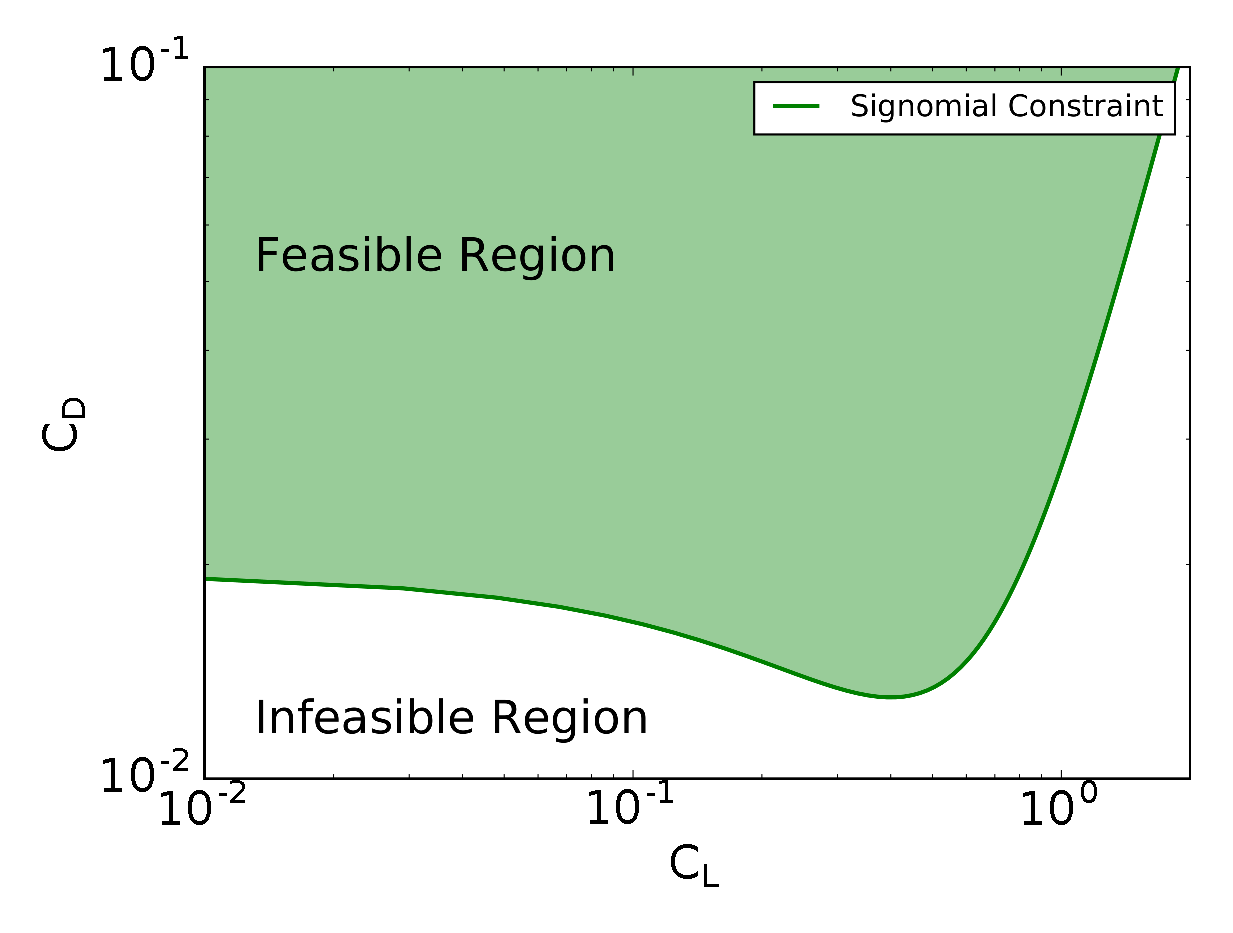
\includegraphics[width=0.45\textwidth]{posyapprox0.eps}}\hfill
%\subfloat[Convex approximation about $C_{L} = 0.05$.]{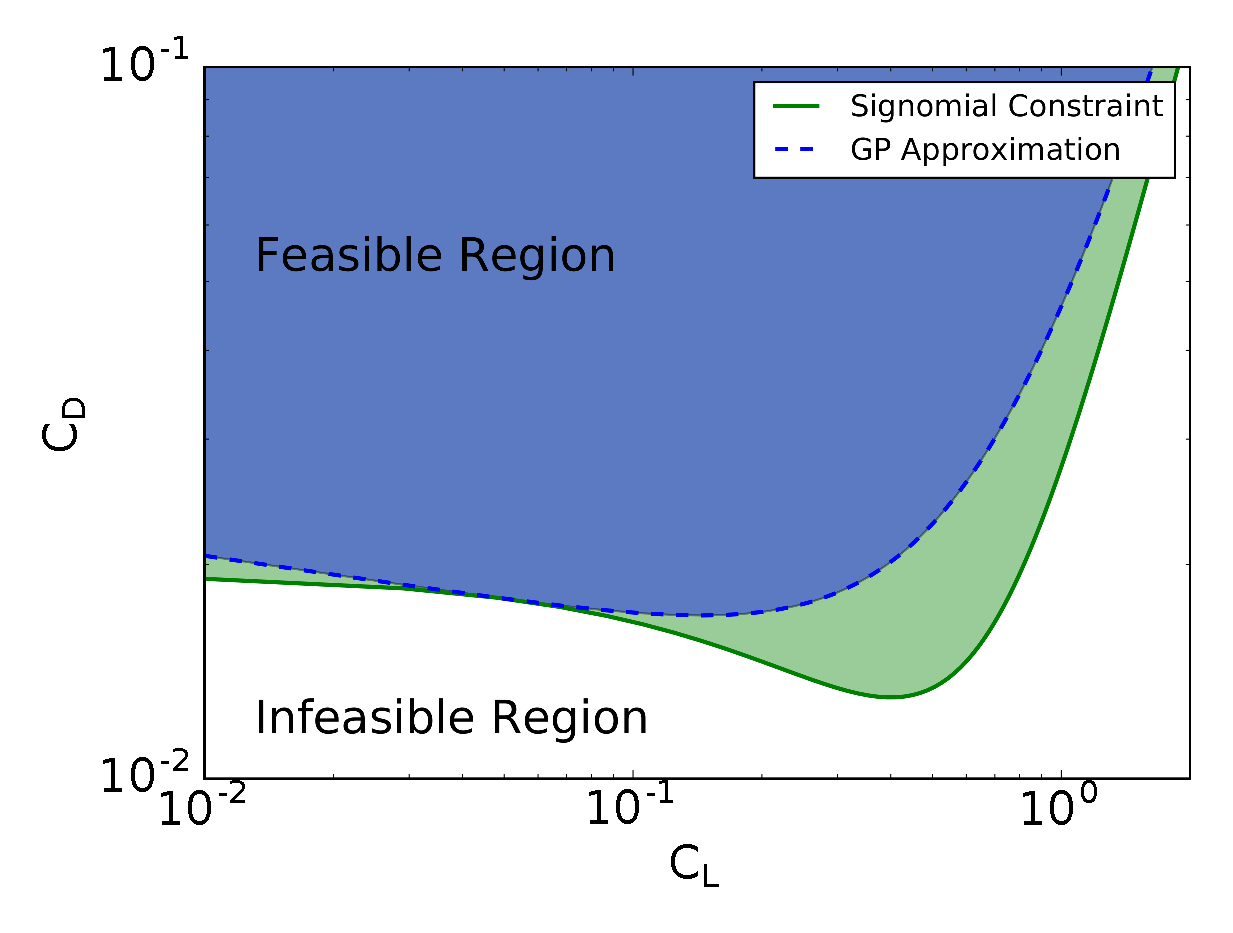
\includegraphics[width=0.45\textwidth]{posyapprox1.eps}}\hfill
%\subfloat[Convex approximation about $C_{L} = 0.20.$]{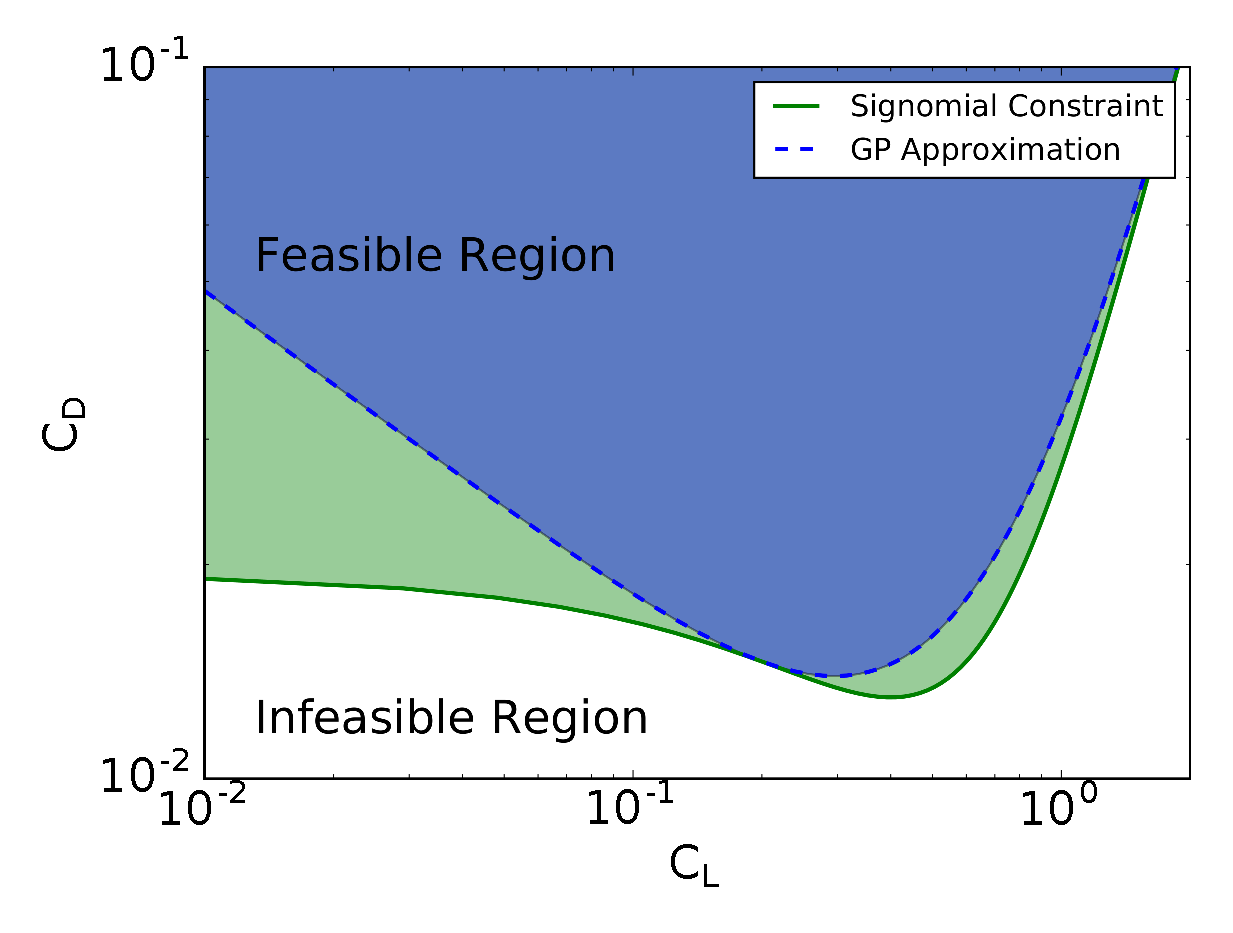
\includegraphics[width=0.45\textwidth]{posyapprox3.eps}}
%\caption{A signomial inequality constraint and GP approximations about two
%different points.} \label{f:GPapproxs}
%\end{figure}

Signomial equality constraints can be approximated by monomials as shown in
Figure \ref{fig:sigeq} and may require a trust region. Trust regions were not
used in the presented model. Signomial equalities are the least desirable type
of constraint due the approximations involved. Most constraints in this work
were relaxed to inequalities and checked for tightness by GPkit\cite{gpkit}. For
additional details on how signomial equalities are approximated, see Opgenoord
et al.\cite{sigeqpaper}.

\begin{figure}[!ht]
\centering
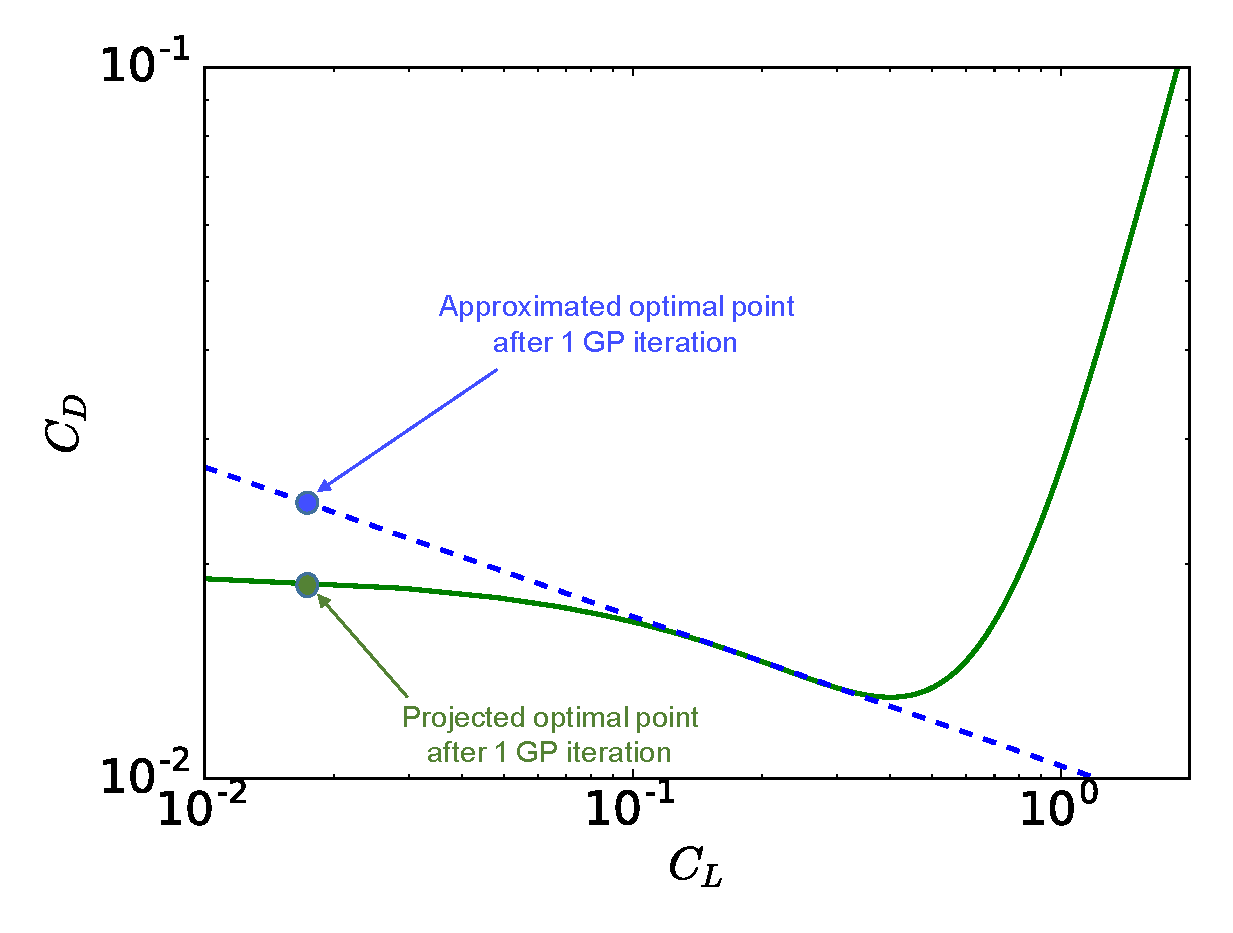
\includegraphics[width=.7\textwidth,natwidth=576,natheight=432]{sigeqapprox.eps}
\caption{The signomial equality constraint $C_{D} = f(C_{L})$ and its
approximation.}\label{fig:sigeq}
\end{figure}


\chapter{Figures}

\vspace*{-3in}

\listoffigures

%% This defines the bibliography file (main.bib) and the bibliography style.
%% If you want to create a bibliography file by hand, change the contents of
%% this file to a `thebibliography' environment.  For more information 
%% see section 4.3 of the LaTeX manual.
\begin{singlespace}
\bibliography{main}
\bibliographystyle{plain}
\end{singlespace}

\end{document}

